\documentclass[12pt]{article} 
\usepackage[utf8]{inputenc}
\usepackage[margin=2.5cm]{geometry} % decrease the margin size

\usepackage{hyperref} % to include weblinks

\usepackage{graphicx} % handle images and figures
\usepackage{placeins} % to control placement of figures
\usepackage{subcaption}
\usepackage{wrapfig}

\usepackage{amsmath} % general package for writing math
\usepackage{amsfonts} % math fonts for obscure symbols

\usepackage[version=4]{mhchem} % chemistry notation

\usepackage[nottoc]{tocbibind}
\usepackage[backend=biber,dateabbrev=false]{biblatex} % package for handling references
\addbibresource{references.bib}
\usepackage{csquotes}

\usepackage{fancyhdr}

\usepackage{siunitx}

\usepackage{multicol}

\setlength{\parindent}{0pt} % remove indentation at the beginning of pargraphs

\begin{document}

\pagestyle{fancy}
\setlength{\headheight}{15pt}
\fancyhead[L]{Infrared Spectroscopy}
\fancyhead[R]{Louis-Hendrik Barboutie, Rajon Bhuyan}


\begin{titlepage}
    \begin{center}
        \vspace*{1cm}
        \Huge
        \textbf{Infrared Spectroscopy}
        
        \vspace{0.5cm}
        \LARGE
        Physikalisches Praktikum für Fortgeschrittene I
        
        \vspace{1.5cm}
        \textbf{Louis-Hendrik Barboutie and Rajon Bhuyan} \newline
        \textbf{7016306 \& 7029677}
        
        \vspace{0.5cm}
        \Large 
        Supervisor: Dr. Klaus Schappert
        
        \vfill

        \includegraphics[width=0.4\textwidth]{logo_uni.png}
        
        \Large
        $27^{\underline{\text{th}}}$ January 2023
    \end{center}
\end{titlepage}

\tableofcontents
\newpage

\section{Introduction}
Infrared spectroscopy has found wide applicability in the area of analytical chemistry for the use in substance identification and quality control. It allows to reliable identify characteristic groups in molecules, and by using various techniques it allows to identify whole molecules. When being confronted to an unknown sample, one can refer to ever growing databases of spectra of pure compounds to identify their sample. 

In addition to identification purposes, infrared spectroscopy can also give quantitative information about samples. Because it is not restrained to solids only, it can be used to determine concentrations of solutes in liquid samples (by using the Beer-Lambert law).

Using quantum mechanical models of the harmonic oscillator and rotor, it is possible to characterize the properties of the chemical bonds in a molecule.

Further applications include the study of phase transitions, as the infrared spectrum is very sensible to the temperature. It enables the determination of the critical temperatures at which the phase transitions occur.

The diverse applications of infrared spectroscopy has made it a tool used in a wide range of fields, both in research and industry.

\section{Theory}

\subsection{IR frequency range:} 300 GHz - 430 THz \cite{InfraredWikipedia}, corresponding to wavelengths of 700 nm - 1 mm. It is divided into three sections: near-, mid- and far-infrared regions. The mid-infrared region is the one which is of interest in this experiment and corresponds to wave numbers of 5000 \si{cm^{-1}} to 300 \si{cm^{-1}} 

\subsection{IR sources} 
Natural infrared light radiation sources are stars \cite{NASAInfrared}, but it is possible to detect an infrared signature from other objects by the mean of black-body radiation \cite{BlackBodyRadiationWikipedia}.
Infrared light for use in spectroscopy can be generated by a tungsten halogen lamp, a heated silicon-carbide element, or a mercury discharge lamp, respectively covering the frequency ranges for near-, mid- and far-infrared light \cite{FourierTransformInfraRedSpectroscopy}. 

\subsection{Prerequisites for IR-activity}
In order to have IR-active oscillations, the molecules must be able to interact with electromagnetic waves, they must have a magnetic dipole. Oscillations where there is no magnetic dipole cannot be detected, when for example the charge center overlaps. This makes it impossible to observe gases like \ce{H2} or \ce{N2} with IR spectroscopy.

\subsection{IR detectors:} Uncooled indium gallium arsenide photodiodes can be used as detectors for the near-infrared, whereas liquid nitrogen cooled mercury cadmium telluride for the mid-infrared and thermally sensible pyroelectric detectors, like deuterated triglycine sulfate or lithium tantalate, for the far-infrared. 

\subsection{Recording the transmission of a sample:}

The first step is to record a background spectrum. This gives us the background intensity as a function of the wave number: $I_0 (\overline{\nu})$.

The second step is to record the spectrum with the sample inside the chamber. This gives us again the intensity as a function of the wave number: $I(\overline{\nu})$.

The \textit{transmission percentage} $T_\%$ is then obtained by dividing both quantities:
\begin{equation}
    \boxed{T_\% = \frac{I}{I_0} \cdot 100}
    \label{eq:IRTransmission}
\end{equation}

\subsection{Lorentzian Functions:}

A \textit{Lorentzian function} $L_i(x)$ with its peak in $x_i$ is described by the equation
\begin{equation}
    \boxed{L_i(x) = y_i + \frac{2 A_i}{\pi} \cdot \frac{\Gamma_i}{4(x - x_i)^2 + \Gamma_i^2}}
\end{equation}
where $\Gamma_i$  is the full width at half maximum, and $A_i$ the area under the curve and $y_i$ the offset. When we fit several Lorentzians at once, we get the sum of the functions as
\begin{equation}
    L(x) = \sum_i \left[ y_i + \frac{2 A_i}{\pi} \cdot \frac{\Gamma_i}{4(x - x_i)^2 + \Gamma_i^2} \right]
\end{equation}

\subsection{Energy levels of quantum mechanical oscillator:}
The allowed energy levels are \cite{SakuraiModernQuantumMechanics}
\begin{equation}
    E_n = \left( n + \frac{1}{2} \right) \hbar \omega, \quad n \in \mathbb{N}
\end{equation}
where $n$ is the quantum number giving the energy level, and $\omega$ the angular frequency of the oscillator.

\subsection{Energy levels of quantum mechanical rotator:}
For a moment of inertia $I$, reduced mass $\mu$ and the distance $r$ separating the two rotating masses, linked together by the relation 
\begin{equation}
    I = \mu r^2
\end{equation}
the allowed energy levels of the rigid rotor are \cite{RigidRotorWikipedia}
\begin{equation}
    E_l = \frac{\hbar^2}{2 I} l(l+1), \quad l \in \mathbb{N}
\end{equation}
Defining the rotation constant as $B = \frac{\hbar}{4 \pi c I}$, this becomes
\begin{equation}
    E_l = B h c l(l+1)
\end{equation}
The moment of inertia is related to the rotation constant in the following way:
\begin{equation}
    I = \frac{\hbar}{4 \pi c B}
\end{equation}

When considering the non-rigid rotor,  the allowed energy levels are
\begin{equation}
    E_l = B h c [ l ( l + 1 ) ] - D h c [l (l+1)]^2
\end{equation}
where $D = \frac{4 B^3}{w^2}$ and $w = \frac{1}{2 \pi c} \sqrt{\frac{k}{\mu}}$, with $k$ the force constant (or bond strength) of the two masses, and $\mu$ the reduced mass.

A change of energy $\Delta E$ is only allowed for $\Delta l = \pm 1$. 

\subsection{Energy levels of quantum mechanical oscillator and rotor combined:}
The total energy is the sum of the energies from the harmonic oscillator and from the rotor:
\begin{equation}
    E_{n+l} = \left( n + \frac{1}{2} \right) hc \overline{\nu}_0 + B hc l(l+1)
\end{equation}

The wave number $\overline{\nu}$ of the photon corresponding to a given transition is given by the relation:
\begin{equation}
    \overline{\nu} = \frac{\Delta E_{n,l}}{h c}
\end{equation}
The spectrum of such  as system shows regions which can be distinguished by the transition of $n$. Each of these regions can again be distinguished into two regions, the $P$ band and the $R$ band, which correspond to the $l$ transitions.
Under consideration that the rotation and stretching constants are not equal for a given $n$, for a combined non-rigid harmonic oscillator and rotor this relation becomes:
\begin{equation}
    \overline{\nu} = \overline{\nu}_0 + B_1[l'(l' + 1)] - D_1[l'(l' + 1)]^2 - B_0[l''(l'' + 1)] + D_0[l''(l'' + 1)]^2
\end{equation}
Here we consider the transition from $n= 0 \rightarrow 1$. We can then use that the $R$ band peaks correspond to $l' = l'' + 1$ and the $P$ band peaks correspond to $l' = l'' - 1$ to deduce the relations:
\begin{equation}
    \Delta \overline{\nu}_0 = \frac{R_{l-1} - P_{l+1}}{2l+1} = (2 B_0 - 3 D_0) - D_0 (2l + 1 )^2
\end{equation}
\begin{equation}
    \Delta \overline{\nu}_1 = \frac{R_{l} - P_{l}}{2l+1} = (2 B_1 - 3 D_1) - D_1 (2l + 1 )^2
\end{equation}

Similarly, we get for the transition $n = 1 \rightarrow 2$ the relations:
\begin{equation}
    \Delta \overline{\nu}_0 = \frac{R_{l-1} - P_{l+1}}{2l+1} = (2 B_0 - 3 D_0) - D_0 (2l + 1 )^2
\end{equation}
\begin{equation}
    \Delta \overline{\nu}_2 = \frac{R_{l} - P_{l}}{2l+1} = (2 B_2 - 3 D_2) - D_2 (2l + 1 )^2
\end{equation} 


\subsection{Refractive index of a sample:}
Multiple reflection can occur at the boundaries of the sample. In the interferogram, this translates to additional bursts symmetrically around the main center burst. The refractive index of the sample can then be deduced with the equation
\begin{equation}
    n = \frac{x_i \lambda_{laser}}{2d}
    \label{eq:InterferogramRefractiveIndex}
\end{equation}
where $d$ is the thickness of the sample and $x_i$ the position of the additional bursts.

Another method to determine the refractive index is to exploit the oscillations in the baseline, which are produced by the multiple reflections. The transmission can be described by 
\begin{equation}
    T = \frac{(1-R)^2}{(1-R^2) + 4R \sin^2\left( \frac{\delta}{2} \right)} \ , \quad \text{with} \ R = \left( \frac{n-1}{n+1} \right)^2 \quad \text{and} \ \delta = \frac{4 \pi n d}{\lambda} 
\end{equation}

The oscillation in the transmission has a maximum when the sine vanishes, or equivalently, when 
\begin{equation}
    \frac{\delta}{2} = m \pi \ , \quad m \in \mathbb{Z}
\end{equation}
This is equivalent to 
\begin{equation}
    \frac{2 \pi n d}{\lambda_m} = m \pi 
\end{equation}
With $\lambda_m = \frac{1}{\overline{\nu}_m}$ the oscillation wavelength of the sine
Finally, we obtain:
\begin{equation}
    n = \frac{m}{2d \overline{\nu}_m}
    \label{eq:SpectrumRefractiveIndex}
\end{equation}

\newpage
\subsection{Structural and condensed molecular formulae}

\begin{figure}[!ht]
    \begin{subfigure}[c]{0.5\textwidth}
        \centering
        \includegraphics[width=0.6\textwidth]{4_Infrared/Graphics/Results/1_1_Sample Identification/CelluloseAcetateButyrate.png}
        \caption{Cellulose Acetate Butyrate}
    \label{fig:StructureCelluloseAcetateButyrate}
    \end{subfigure}
    \hfill
    \begin{subfigure}[c]{0.5\textwidth}
        \centering
        \includegraphics[width=0.6\textwidth]{4_Infrared/Graphics/Results/1_1_Sample Identification/CelluloseTriacetate.png}
        \caption{Cellulose Triacetate}
    \label{fig:StructureCelluloseTriacetate}
    \end{subfigure}
    \hfill
    \begin{subfigure}[c]{0.5\textwidth}
        \centering
        \includegraphics[width=0.6\textwidth]{4_Infrared/Graphics/Results/1_1_Sample Identification/Kapton.png}
        \caption{Kapton}
    \label{fig:StructureKapton}
    \end{subfigure}
    \hfill
    \begin{subfigure}[c]{0.5\textwidth}
        \centering
        \includegraphics[width=0.6\textwidth]{4_Infrared/Graphics/Results/1_1_Sample Identification/PolyCarbonate.png}
        \caption{Polycarbonate}
    \label{fig:StructurePolycarbonate}
    \end{subfigure}
    \hfill
    \begin{subfigure}[c]{0.5\textwidth}
        \centering
        \includegraphics[scale=0.1]{4_Infrared/Graphics/Results/1_1_Sample Identification/Polystyrol.png}
        \caption{Polystyrol}
    \label{fig:StructurePolystyrol}
    \end{subfigure}
    \hfill
    \begin{subfigure}[c]{0.5\textwidth}
        \centering
        \includegraphics[width=0.6\textwidth]{4_Infrared/Graphics/Results/1_1_Sample Identification/Teflon.png}
        \caption{Teflon}
    \label{fig:StructureTeflon}
    \end{subfigure}
    \caption{Molecular structures of the sample materials}
    \label{fig:MolecularStructures}
\end{figure}
 \FloatBarrier
 
\newpage
\section{Experimental Setup}
The IR spectrometer present in the lab generates IR radiation with a source made of silicon carbide, which is heated to about 1000 \si{\kelvin} and emits radiation similar to a black body. Using an interferometer it records and inteferogram, which is then fourier-transformed to obtain the spectrum. The functioning is sketched in fig.~\ref{fig:SchematicFTIRSpectrometer} \cite{FTIR_Schematic}.

\begin{figure}[!ht]
    \centering
    \includegraphics[width=0.7\textwidth]{4_Infrared/Graphics/Setup/Fourier_transform_spectrometer.png}
    \caption{Schematic of the Fourier-Transform IR Spectrometer}
    \label{fig:SchematicFTIRSpectrometer}
\end{figure}
\FloatBarrier

The procedure for recording IR spectra with the device in fig.~\ref{fig:IRSpectrometer} is rather simple: it mainly consists of two steps. The first one is to record the background spectrum, without the sample we want to study. Then the second step is to introduce the sample and record the spectrum. The software automatically computes the transmission given by eq.~\ref{eq:IRTransmission}, and gives the transmission spectrum.

For the recording of the background there are filters available, which smooth out the signal from the water and carbon dioxide naturally present in the air. For a similar reason, when studying some compounds, it is of interest to do so in vacuum, so as to not get unwanted signal. This is done when studying the phase transition of an alkane in the last part of this experiment.

\begin{figure}[ht]
    \begin{subfigure}[c]{0.5\textwidth}
        \centering
        \includegraphics[width=\textwidth]{4_Infrared/Graphics/Setup/IRSpectrometer.jpg}
        \caption{IR-Spectrometer}
        \label{fig:IRSpectrometer}
    \end{subfigure}
    \hfill
    \begin{subfigure}[c]{0.5\textwidth}
        \centering
        \includegraphics[width=\textwidth, angle=-90]{4_Infrared/Graphics/Setup/ThicknessMeasurer.jpg}
        \caption{Thickness measurement device}
    \end{subfigure}
    
    \begin{subfigure}[c]{0.32\textwidth}
        \centering
        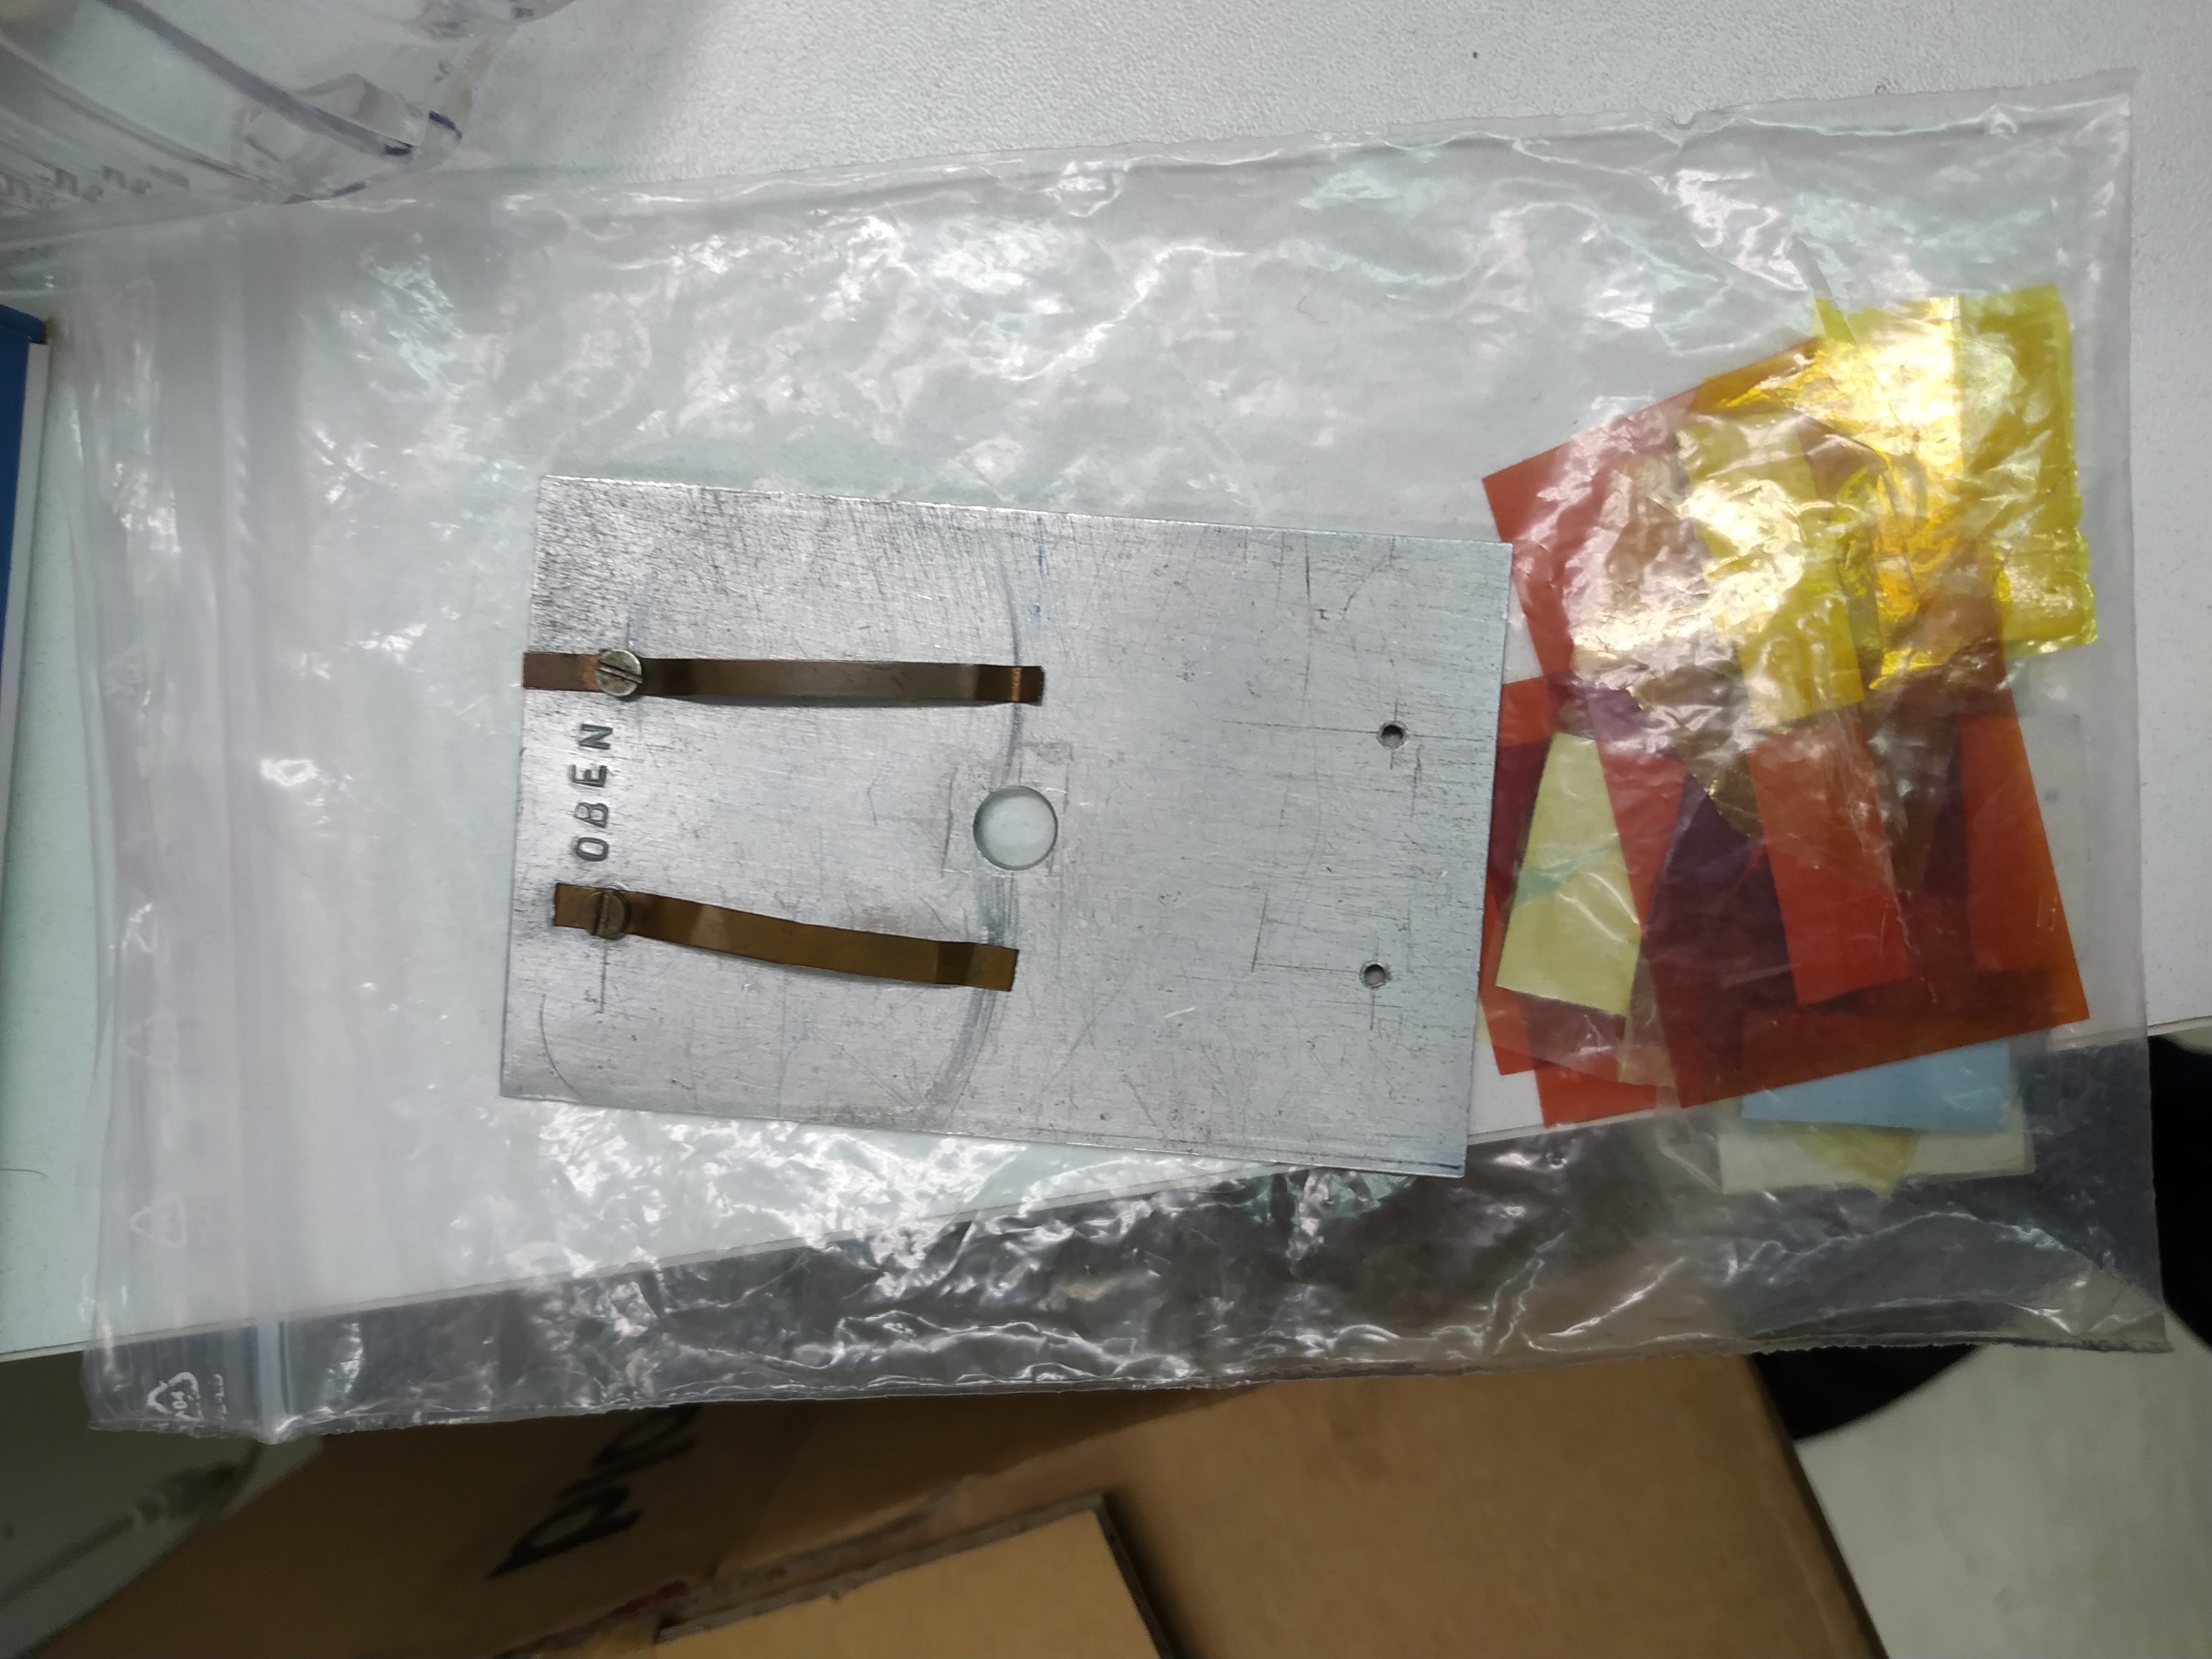
\includegraphics[width=\textwidth, angle=-90]{4_Infrared/Graphics/Setup/Samples.jpg}
        \caption{Sample holder and provided samples}
    \end{subfigure}
    \hfill
    \begin{subfigure}[c]{0.32\textwidth}
        \centering
        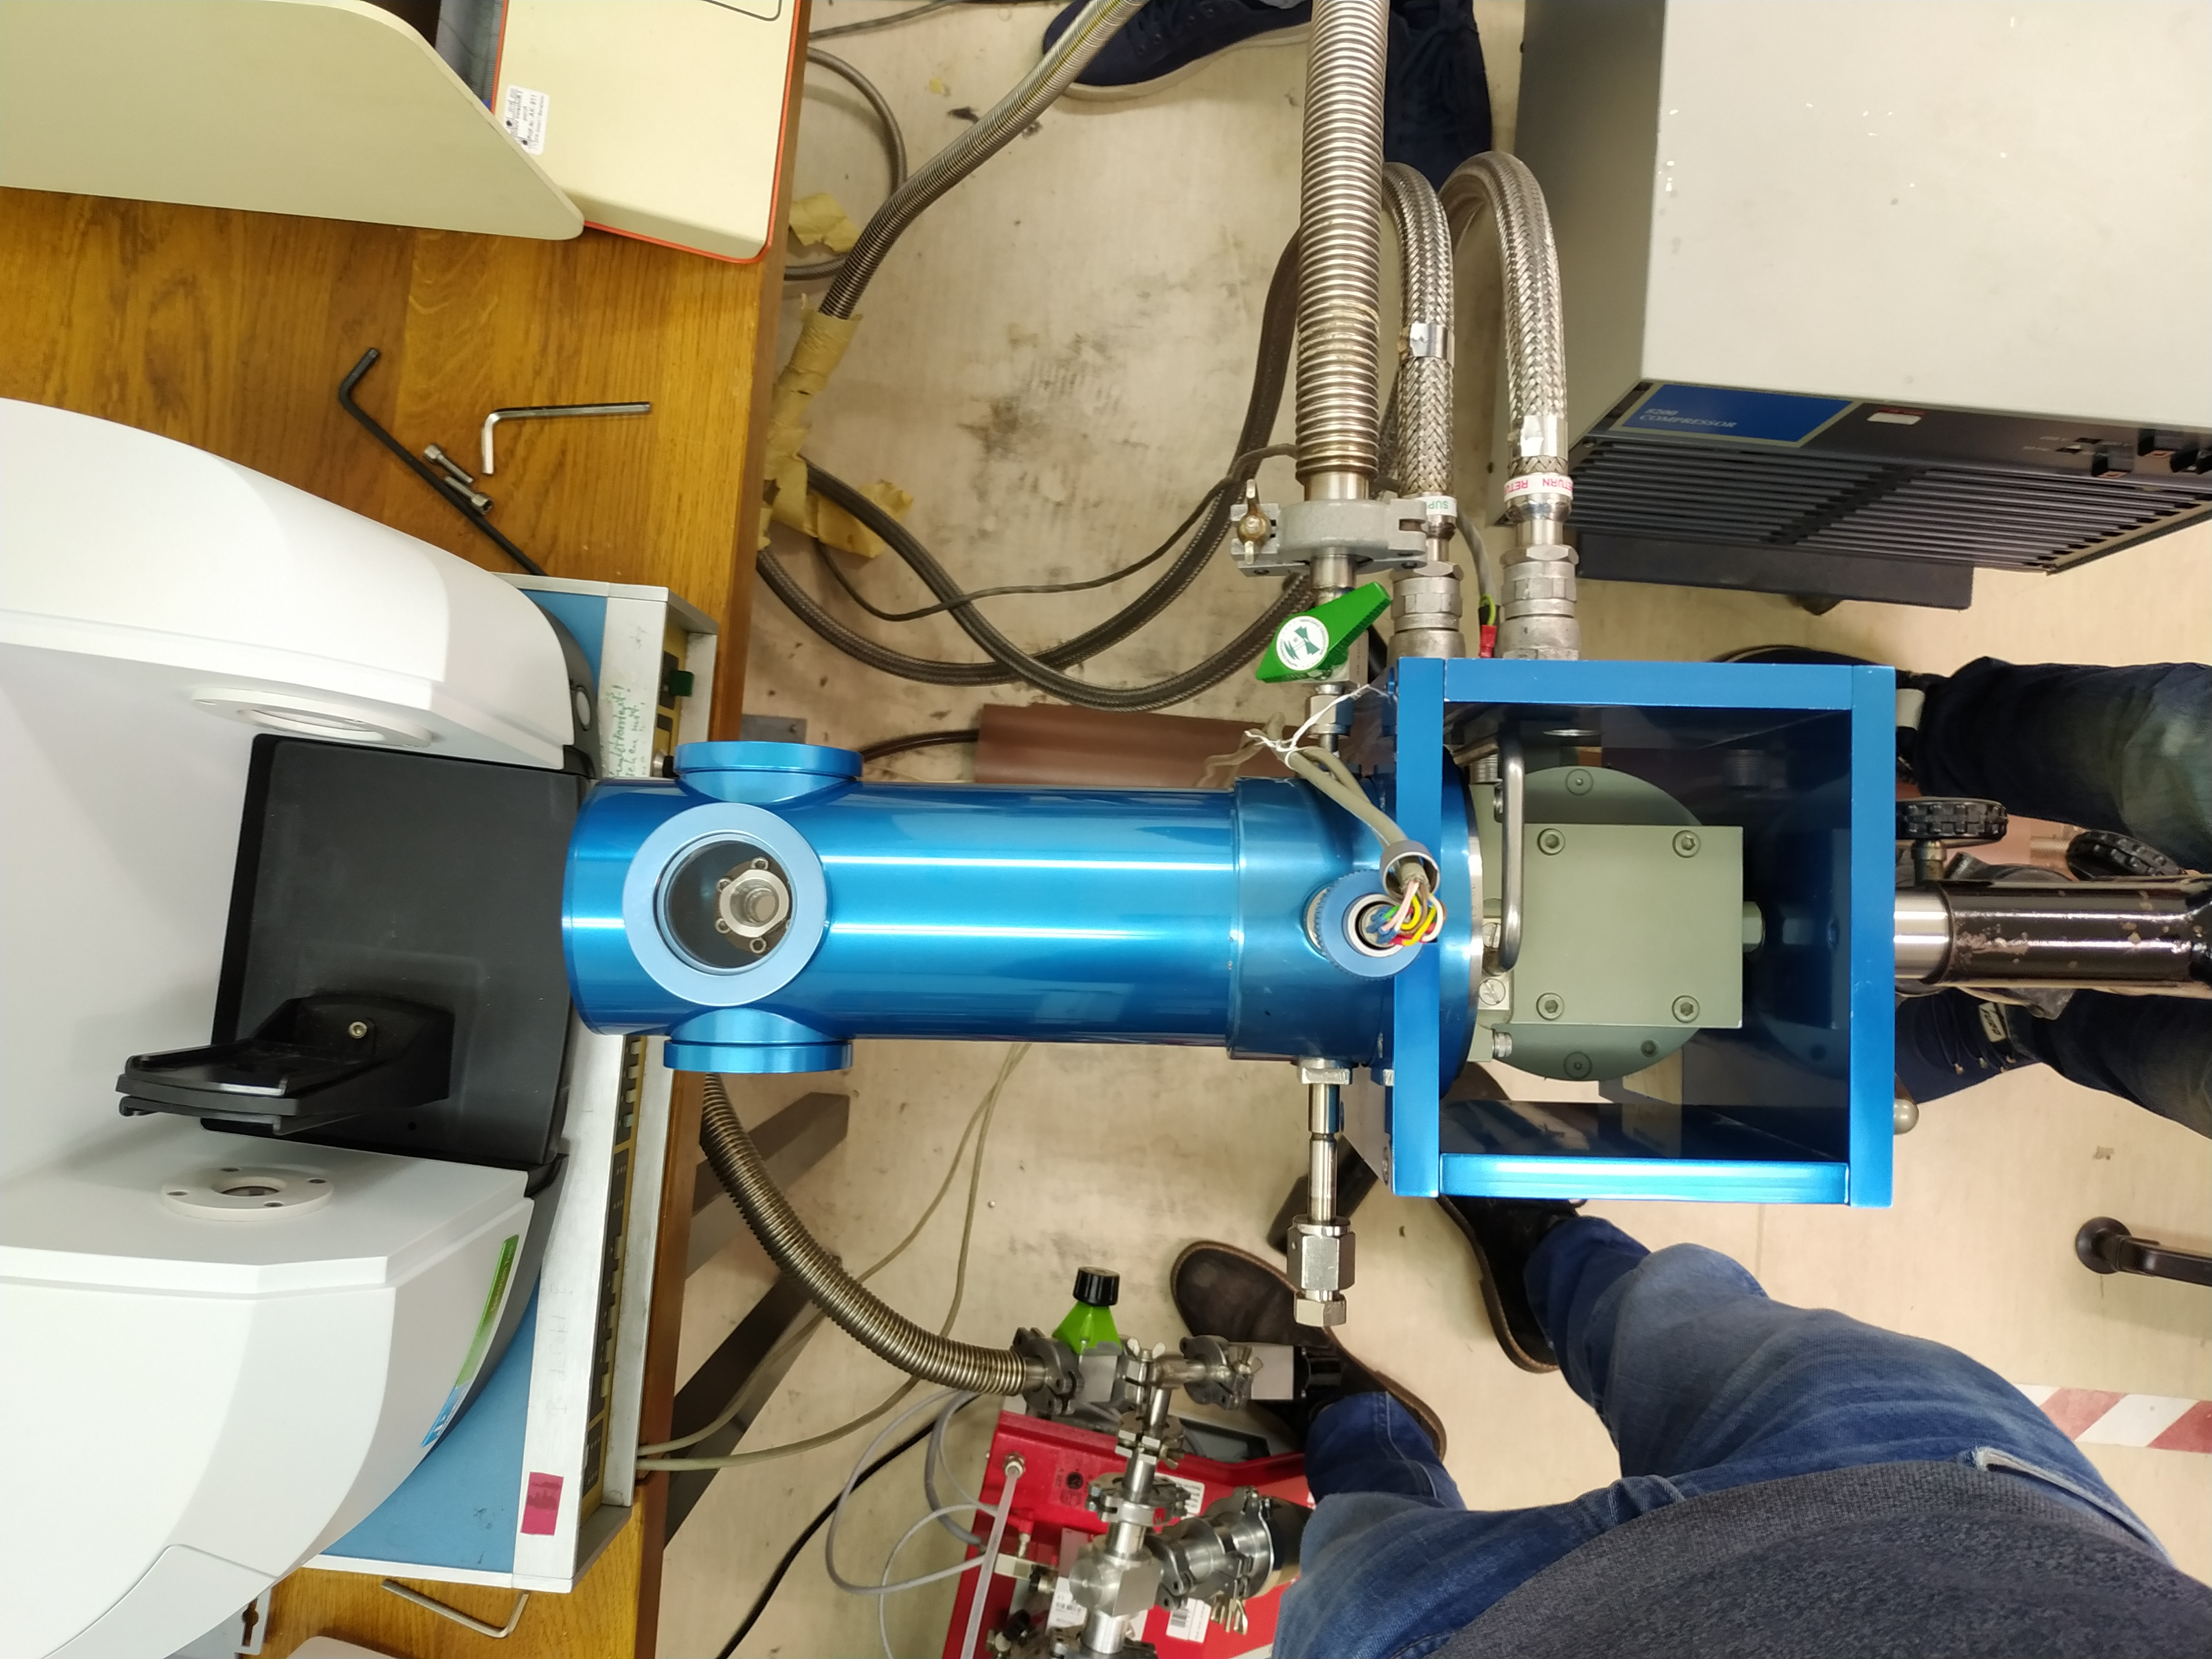
\includegraphics[width=\textwidth, angle=-90]{4_Infrared/Graphics/Setup/SampleChamberAlkane.jpg}
        \caption{Vacuum chamber with an alkane sample}
    \end{subfigure}
    \hfill
    \begin{subfigure}[c]{0.32\textwidth}
        \centering
        \includegraphics[width=\textwidth, angle=-90]{4_Infrared/Graphics/Setup/SampleChamberCarbonMonoxide.jpg}
        \caption{Chamber containing carbon monoxide}
    \end{subfigure}
    \caption{Experimental Devices}
    \label{fig:ExperimentalDevices}
\end{figure}
\FloatBarrier

\newpage

\section{Results}

\subsection{Filtering out unwanted signal}

When we record the background intensity, we have the option to apply a filter for dihydrogen monoxide (\ce{H2O}) and carbon dioxide (\ce{CO2}), which are naturally present in the ambient air. As can be seen in fig. \ref{fig:KBrBackgroundSpectraComparison}, the peaks in the ranges 3950 cm$^{-1}$ to 3500 cm$^{-1}$, 2400 cm$^{-1}$ to 2300 cm$^{-1}$ and 2000 cm$^{-1}$ to 1300 cm$^{-1}$ , corresponding to \ce{H2O} and \ce{CO2} are smoothed out, although no perfectly. This process removes excess noise in these ranges in the subsequent spectra.

\begin{figure}[!ht]
    \begin{subfigure}[t]{0.5\textwidth}
        \centering
        \includegraphics[width=\textwidth]{4_Infrared/Graphics/Results/1_0_Background Filter/BackgroundSpectrumKBrWindowWithoutFilter.png}
        \caption{Inactive filter}
        \label{fig:KBrBackgroundWithoutFilter}
    \end{subfigure}
    \hfill
    \begin{subfigure}[t]{0.5\textwidth}
        \centering
        \includegraphics[width=\textwidth]{4_Infrared/Graphics/Results/1_0_Background Filter/BackgroundSpectrumKBrWindowWithFilter.png}
        \caption{Active filter}
        \label{fig:KBrBackgroundWithFilter}
    \end{subfigure}
    \caption{Comparison of background spectra with and without \ce{H2O}/\ce{CO2} filter}
    \label{fig:KBrBackgroundSpectraComparison}
\end{figure}
\FloatBarrier

\subsection{Sample identification}

\subsubsection{Possible Materials}

Each of the unknown samples is made out of the following materials:
\begin{itemize}
    \item Cellulose Acetate Butyrate
    \item Cellulose Triacetate
    \item Kapton
    \item Polycarbonate
    \item Polystyrol
    \item Teflon
\end{itemize}

The molecular structures are shown in fig. \ref{fig:MolecularStructures}. It is possible to identify characteristic groups for some molecules: teflon is the only molecule containing fluoride and kapton the only molecule containing nitrogen. polycarbonate, polystyrol and cellulose acetate butyrate contain benzene rings, whereas cellulose triacetate and teflon do not. 

\subsubsection{Sample 1}
\begin{wrapfigure}[18]{R}{0.6\textwidth}
    \centering
    \includegraphics[width=0.6\textwidth]{4_Infrared/Graphics/Results/1_1_Sample Identification/SpectrumIdentifiedTeflon.png}
    \caption{Spectrum of sample 1}
    \label{fig:SpectrumIdentifiedTeflon}
\end{wrapfigure}
The spectrum obtained for sample 1 is shown in fig. \ref{fig:SpectrumIdentifiedTeflon}. We can immediately identify it as the teflon sample, as it shows the characteristic peak for \ce{CF2} and \ce{CF3} bonds in the range 1150 cm$^{-1}$ to 1250 cm$^{-1}$. There are also peaks in the region from 680-780 \si{cm^{-1}} which correspond to \ce{CF3} oscillations. As expected for teflon, there is an absence of peaks for oscillations in benzene rings of of carbon-oxygen bonds. Since we know each sample is different, we can exclude every following sample as being teflon. We can see that the baseline follows some kind of sine wave. 



\subsubsection{Sample 3}
\begin{wrapfigure}{R}{0.6\textwidth}
    \centering
    \includegraphics[width=0.6\textwidth]{4_Infrared/Graphics/Results/1_1_Sample Identification/SpectrumIdentifiedKapton.png}
    \caption{Spectrum of sample 3}
    \label{fig:SpectrumIdentifiedCelluloseAcetateButyrate}
\end{wrapfigure}
The spectrum obtained for sample 3 is shown in fig. \ref{fig:SpectrumIdentifiedCelluloseAcetateButyrate}. It is not teflon, as it is missing the characteristic peaks in the regions from 1150 cm$^{-1}$ to 1250 cm$^{-1}$. We can identify traces of benzene rings however, so it cannot be cellulose triacetate or cellulose acetate butyrate. Note that while the baseline exhibits a sinusoidal tendency, the peak for benzene is a sharp cutoff and therefore not just another oscillation of the baseline. Since we there is a characteristic peak for a carbon-oxygen-carbon structure, it cannot be polystyrol either. Since there's a peak for \ce{NC3}, the sample has to contain kapton.

\newpage
\subsubsection{Sample 6}
\begin{wrapfigure}[18]{r}{0.6\textwidth}
    \centering
    \includegraphics[width=0.7\textwidth]{4_Infrared/Graphics/Results/1_1_Sample Identification/SpectrumIdentifiedCelluloseTriacetate.png}
    \caption{Spectrum of sample 6}
    \label{fig:SpectrumIdentifiedCelluloseTriacetate}
\end{wrapfigure}
The spectrum obtained for sample 6 is shown in fig. \ref{fig:SpectrumIdentifiedCelluloseTriacetate}. We can exclude it being teflon or kapton, as it does not have the characteristic peaks in the regions from 1150 cm$^{-1}$ to 1250 cm$^{-1}$ and from 1265 cm$^{-1}$ to 1380 cm$^{-1}$. As we can identify carbon-oxygen bonds, we can exclude the sample to be polystyrol. The transmission floors in the region from 1000 \si{cm^{-1}} to 1500 \si{cm^{-1}}, which corrsepond to vibrations of the carbon-oxygen bonds, which are plentiful in cellulose triacetate or in cellulose acetate butyrate. There is no characteristic peak for benzene rings, so by using the exclusion principle, the sample can only contain cellulose triacetate. 



\subsection{Alkane chain length determination}

Since Alkanes are only composed of \ce{CH2} and \ce{CH3}, the resulting spectrum contains transmission peaks in the region from 3000 cm$^{-1}$ to 2800 cm$^{-1}$. There are four peaks in total, corresponding to both symmetric and asymmetric oscillations, which produce peaks with a slight shift. In addition to the four expected peaks, one also has to consider a fifth one corresponding to \ce{CH} oscillations.

We can compare the chain lengths of the alkanes by looking at the ratio
\begin{equation}
    A = \frac{T(\ce{CH2})}{T(\ce{CH3})}
\end{equation}
By considering this ratio, we eliminate the concentration dependency of the spectrum, as each sample has different amounts of alkanes inside of them. We can identify the couple of peaks with higher wave number as the asymmetrical oscillations, and the couple of peaks with smaller wave number as the symmetrical oscillations. The longer an alkane is, the more \ce{CH2} oscillations there are, therefore the total area of \ce{CH2} increases with the length. Greater values of $A$ indicate longer alkanes. Since the peaks are Lorentzians and not delta shaped, we compare their area and not the maxima. The formula for $A$ then becomes:
\begin{equation}
    A = \frac{A_{asym}(\ce{CH2}) + A_{sym}(\ce{CH2})}{A_{asym}(\ce{CH3}) + A_{sym}(\ce{CH3})}
\end{equation}

\begin{figure}[!ht]
    \centering
    \includegraphics[width=0.7\textwidth]{4_Infrared/Graphics/Results/1_2_Alkane Chain Length/SpectrumZoomedFittedU1.png}
    \caption{Fitted Spectrum of the Alkane sample U1}
    \label{fig:FittedSpectrumU1}
\end{figure}
\FloatBarrier

\begin{figure}[!ht]
    \centering
    \includegraphics[width=0.7\textwidth]{4_Infrared/Graphics/Results/1_2_Alkane Chain Length/SpectrumZoomedFittedU2.png}
    \caption{Fitted Spectrum of the Alkane sample U2}
    \label{fig:FittedSpectrumU2}
\end{figure}
\FloatBarrier

\begin{figure}[!ht]
    \centering
    \includegraphics[width=0.7\textwidth]{4_Infrared/Graphics/Results/1_2_Alkane Chain Length/SpectrumZoomedFittedU3.png}
    \caption{Fitted Spectrum of the Alkane sample U3}
    \label{fig:FittedSpectrumU3}
\end{figure}
\FloatBarrier

\begin{figure}[!ht]
    \centering
    \includegraphics[width=0.7\textwidth]{4_Infrared/Graphics/Results/1_2_Alkane Chain Length/SpectrumZoomedFittedG1.png}
    \caption{Fitted Spectrum of the Alkane sample G1}
    \label{fig:FittedSpectrumG1}
\end{figure}
\FloatBarrier

\begin{figure}[!ht]
    \centering
    \includegraphics[width=0.7\textwidth]{4_Infrared/Graphics/Results/1_2_Alkane Chain Length/SpectrumZoomedFittedG2.png}
    \caption{Fitted Spectrum of the Alkane sample G2}
    \label{fig:FittedSpectrumG2}
\end{figure}
\FloatBarrier

\begin{table}[!ht]
    \centering
    \begin{tabular}{|c|c|}
    \hline
        Sample & $A$ \\ \hline \hline
        G1 & $(2,21 \pm 0,22)$ \\ \hline
        G2 & $(2,47 \pm 0,13)$ \\ \hline
        U1 & $(3,55 \pm 0,18)$  \\ \hline
        U2 & $(4,12 \pm 0,36)$  \\ \hline
        U3 & $(2,20 \pm 0,10)$  \\ \hline
    \end{tabular}
    \caption{Ratios of the asymmetric and symmetric oscillation transmission ratios for the five samples}
    \label{tab:AlkaneChainLengthValues}
\end{table}
The uncertainty on the area has been extracted from the fitting process.
Since the smaller $A$, the shorter the alkane, we deduce the following order for the length of the samples: U3 $<$ G1 $<$ G2 $<$ U1 $<$ U2.

\subsection{Determination of the refractive index}

In this section we determine the refractive index of kapton by two different methods.

\subsubsection{Using the interferogram}

We stacked 4 kapton plates to get better signal, but the result should be the same. We measure a single foil in 5 different places and obtain an average thickness of (135,9 $\pm$ 1,5) $\mu$m. From the interferogram we can find two points in which the signal is retarded: $x_1 = (-542 \pm 5)$ and $x_2 = (543 \pm 5)$. Here the $x_i$ correspond to the distance from the center burst. Using the formula in eq.~\ref{eq:InterferogramRefractiveIndex}, we get an average value of the refractive index of $n= (1,697 \pm 0,035)$.

\begin{figure}[!ht]
    \centering
    \includegraphics[width=\textwidth]{4_Infrared/Graphics/Results/2_RefractiveIndex/Interferogram.png}
    \caption{Interferogram}
    \label{fig:Interferogram}
\end{figure}

\subsubsection{Using the spectrum}
We can obtain the refractive index from oscillations in the baseline of the spectrum via the formula from eq.~\ref{eq:SpectrumRefractiveIndex}, with a slight modification: if we count multiple maxima, it becomes
\begin{equation}
    n = \frac{m}{2d \Delta \overline{\nu}}
\end{equation}
where $m$ is the amount of peaks in the range $\Delta \overline{\nu}$. Using the portion of the spectrum shown in fig.~\ref{fig:SpectrumRefractiveIndex}, we get a value of $n =(1,759 \pm 0,021)$. Here we assume the peak picking is accurate to the half width at half measure of the peak, which is about 2,5 \si{cm^{-1}}.

\begin{figure}[!ht]
    \centering
    \includegraphics[width=\textwidth]{4_Infrared/Graphics/Results/2_RefractiveIndex/SpectrumRefractiveIndex.png}
    \caption{Excerpt from the kapton spectrum with indicated peak positions}
    \label{fig:SpectrumRefractiveIndex}
\end{figure}
\FloatBarrier

Literature values for kapton are $n=1,70$  \cite{DuPontKaptonRefractiveIndex}, this value has been measured with a wavelength of 589 \si{nm}, which may explain the slight difference to our value.

\subsection{Study of carbon monoxide}

\subsubsection{Determination of the rotation and stretching constants}

The full spectrum recorded for carbon monoxide is shown in fig.~\ref{fig:SpectrumFullCO}. There are two areas of interest, which correspond to transitions of the quantum number $n$ from 0 to 1 and from 1 to 2.

\begin{figure}[!ht]
    \centering
    \includegraphics[width=0.7\textwidth]{4_Infrared/Graphics/Results/3_1 Carbon Monoxide/SpectrumFullCO.png}
    \caption{Full spectrum of the CO sample}
    \label{fig:SpectrumFullCO}
\end{figure}
\FloatBarrier

\begin{figure}[!ht]
    \centering
    \includegraphics[width=0.7\textwidth]{4_Infrared/Graphics/Results/3_1 Carbon Monoxide/transitionN01.png}
    \caption{Enlarged spectrum of the $n = 0 \rightarrow 1$ transition}
    \label{fig:SpectrumEnlargedN01}
\end{figure}
\FloatBarrier

\begin{figure}[!ht]
    \centering
    \includegraphics[width=0.7\textwidth]{4_Infrared/Graphics/Results/3_1 Carbon Monoxide/transitionN12.png}
    \caption{Enlarged spectrum of the $n = 1 \rightarrow 2$ transition}
    \label{fig:SpectrumEnlargedN12}
\end{figure}
\FloatBarrier

Enlarging these spectral ranges, we can observe that there is a multitude of single peaks. These correspond to the transitions $\Delta l = \pm 1$. The enlarged spectra are shown in fig.~\ref{fig:SpectrumEnlargedN01} and fig.~\ref{fig:SpectrumEnlargedN12}. There are two bands, the $P$ and the $R$ band, which correspond respectively to a transition $\Delta l = -1$ and $\Delta l = +1$, with a forbidden region in between, which would correspond to $\Delta l = 0$. Each peak can be indexed by $R_l$ or $P_l$, with $l=0,1,2,\dots$ in the $R$ band and $l = 1,2,3, \dots$ in the $P$ band. Furthermore $[R_l] = [P_l] = [\overline{\nu}] =$ cm$^{-1}$

The peak fitting results are presented in fig.~\ref{fig:IndexedBandsN01} and fig.~\ref{fig:IndexedBandsN12}. Note that the index starts at the forbidden region and is therefore in reversed order for the $R$ and $P$ band.
\begin{figure}[!ht]
    \centering
    \begin{subfigure}[c]{0.49\textwidth}
        \centering
        \includegraphics[width=\textwidth]{4_Infrared/Graphics/Results/3_1 Carbon Monoxide/N01_R_Band.png}
        \caption{$R$ band}
    \end{subfigure}
    \hfill
    \begin{subfigure}[c]{0.49\textwidth}
        \centering
        \includegraphics[width=\textwidth]{4_Infrared/Graphics/Results/3_1 Carbon Monoxide/N01_P_Band.png}
        \caption{$P$ band}
    \end{subfigure}
    \caption{Indexed bands for the $n = 0 \rightarrow 1$ transition}
    \label{fig:IndexedBandsN01}
\end{figure}
\FloatBarrier

\begin{figure}[!ht]
    \centering
    \begin{subfigure}[c]{0.49\textwidth}
        \centering
        \includegraphics[width=\textwidth]{4_Infrared/Graphics/Results/3_1 Carbon Monoxide/N12_R_Band.png}
        \caption{$R$ band}
    \end{subfigure}
    \hfill
    \begin{subfigure}[c]{0.49\textwidth}
        \centering
        \includegraphics[width=\textwidth]{4_Infrared/Graphics/Results/3_1 Carbon Monoxide/N12_P_Band.png}
        \caption{$P$ band}
    \end{subfigure}
    \caption{Indexed bands for the $n = 1 \rightarrow 2$ transition}
    \label{fig:IndexedBandsN12}
\end{figure}
\FloatBarrier

Giving a generous error estimate of 0.5 cm$^{-1}$ on the peak position (the error corresponds to the half width at half maximum), we can plot $\Delta \overline{\nu}_0$, $\Delta \overline{\nu}_1$ and $\Delta \overline{\nu}_2$ as shown in fig.~\ref{fig:LinearFitsNuN01} and fig.~\ref{fig:LinearFitsNuN12}.
\begin{figure}[!ht]
    \centering
    \begin{subfigure}[c]{0.49\textwidth}
        \centering
        \includegraphics[width=\textwidth]{4_Infrared/Graphics/Results/3_1 Carbon Monoxide/Nu0_N01.png}
        \caption{Plot of $\Delta \overline{\nu}_0$}
    \end{subfigure}
    \hfill
    \begin{subfigure}[c]{0.49\textwidth}
        \centering
        \includegraphics[width=\textwidth]{4_Infrared/Graphics/Results/3_1 Carbon Monoxide/Nu1_N01.png}
        \caption{Plot of $\Delta \overline{\nu}_1$}
    \end{subfigure}
    \caption{Plots to determine $B_0$, $B_1$, $D_0$, $D_1$}
    \label{fig:LinearFitsNuN01}
\end{figure}
\FloatBarrier

\begin{figure}[!ht]
    \centering
    \begin{subfigure}[c]{0.49\textwidth}
        \centering
        \includegraphics[width=\textwidth]{4_Infrared/Graphics/Results/3_1 Carbon Monoxide/Nu0_N12.png}
        \caption{Plot of $\Delta \overline{\nu}_0$}
    \end{subfigure}
    \hfill
    \begin{subfigure}[c]{0.49\textwidth}
        \centering
        \includegraphics[width=\textwidth]{4_Infrared/Graphics/Results/3_1 Carbon Monoxide/Nu2_N12.png}
        \caption{Plot of $\Delta \overline{\nu}_2$}
    \end{subfigure}
    \caption{Plots to determine $B_0$, $B_2$, $D_0$, $D_2$}
    \label{fig:LinearFitsNuN12}
\end{figure}
\FloatBarrier

We fit them with functions of the form $y = m + x \cdot p$, and obtain:
\begin{table}[!ht]
    \centering
    \resizebox{\textwidth}{!}{
    \begin{tabular}{|c|c|c|c|c|c|c|} \hline
        transition & $B_0$ (cm$^{-1}$) & $B_1$ (cm$^{-1}$) & $B_2$ (cm$^{-1}$) & $D_0$ (cm$^{-1}$) & $D_1$ (cm$^{-1}$) & $D_2$ (cm$^{-1}$) \\ \hline \hline
        $n = 0 \rightarrow 1$ & $(1,92 \pm 0,01)$ & $(1,91 \pm 0,01)$ & / & $(5,66 \pm 0,12) \cdot 10^{-6}$ & $(5,64 \pm 0,12) \cdot 10^{-6}$ & / \\ \hline
        $n = 1 \rightarrow 2$ & $(1,92 \pm 0,02)$ & / & $(1,89 \pm 0,02)$ & $(2,68 \pm 0,34) \cdot 10^{-6})$ & / & $(4,81 \pm 0,28) \cdot 10^{-6}$ \\ \hline
    \end{tabular}
    }
    \caption{Values obtained from the linear fits}
    \label{tab:NuLinearFitValues}
\end{table}
\FloatBarrier

It is striking that the correctional term becomes very small. Using the values of $B$, we can extrapolate to find the value of $B_e$, which corresponds to the rotation without oscillations. The resulting linear relationship is shown in fig.~\ref{fig:BnExtrapolation}. This relationship is expressed by
\begin{equation}
    B_n = B_e - \alpha \left( n + \frac{1}{2} \right)
\end{equation}
From the fit results in fig.~\ref{fig:BnExtrapolation} we obtain $B_e = ( 1,93 \pm 0,03 )$ cm$^{-1}$ as the intercept at origin.

\begin{figure}[!ht]
    \centering
    \includegraphics[width=0.7\textwidth]{4_Infrared/Graphics/Results/3_1 Carbon Monoxide/BnExtrapolation.png}
    \caption{Linear fit of the $B_n$}
    \label{fig:BnExtrapolation}
\end{figure}
\FloatBarrier

\begin{table}[!ht]
    \centering
    \begin{tabular}{|c|c|}
    \hline
        n & $B (\si{cm^{-1}})$ \\ \hline \hline
        e & $(1,93 \pm 0,03)$ \\ \hline
        0 & $(1,92 \pm 0,01)$ \\ \hline
        1 & $(1,91 \pm 0,02)$ \\ \hline
        2 & $(1,89 \pm 0,02)$ \\ \hline
    \end{tabular}
    \caption{Computed and extrapolated rotation constants}
    \label{tab:BnValues}
\end{table}

Literature values are \cite{doi:10.1021/ed073p804}:
\begin{table}[!ht]
    \centering
    \begin{tabular}{|c|c|}
    \hline
        n & $B (\si{10^{-2}cm^{-1}})$ \\ \hline \hline
        e & $(193,81 \pm 1,06)$ \\ \hline
        0 & $(192,93 \pm 1,06)$ \\ \hline
        1 & $(190,60 \pm 0,51)$ \\ \hline
        2 & $(188,86 \pm 0,51)$ \\ \hline
    \end{tabular}
    \caption{Literature value of the constants}
    \label{tab:BnLiteratureValues}
\end{table}
\FloatBarrier
Our values fall well into the given error bounds.

\subsubsection{Determination of the moment of inertia and average bond length}

The calculated moments of inertia for $n \geq 0$ as well as the extrapolated moment of inertia for the state devoid of oscillations are shown in fig.~\ref{fig:MomentsOfInertiaCO} and presented in tab.~\ref{tab:MomentOfInertiaAndBondLengthValues}.

\begin{figure}[!ht]
    \centering
    \includegraphics[width=0.7\textwidth]{4_Infrared/Graphics/Results/3_1 Carbon Monoxide/MomentOfInertiaCO.png}
    \caption{Calculated moments of inertia}
    \label{fig:MomentsOfInertiaCO}
\end{figure}
\FloatBarrier

Since the moment of inertia is defined as in eq.~\ref{eq:MomentOfInertiaDef} and we have no reason to assume it the same for each energy level of $n$, we compute it for each $n$ as:
\begin{equation}
    I_n = \mu r_n^2
    \label{eq:MomentOfInertiaDef}
\end{equation}
with $\mu$ the reduced mass of the system, we can deduce the distance separating the carbon and oxygen atom.
Using the values of $m_C = 1.99 \cdot 10^{-26}$ kg and $m_O = 2.66 \cdot 10^{-26}$, we get a reduced mass of $\mu = 1.14 \cdot 10^{-26}$ kg. The calculated bond lengths are shown in fig.~\ref{fig:BondLengthCO}. We can observe an increase in the bond length for a growing moment of inertia, which correspond to smaller values of $B_n$ and thus higher values of $n$. As the oscillator transitions into higher excited states, the bond length increases. We observe bond length of the order of $10^{-10}$ m, which is typical for a molecular bond length. 
\begin{figure}[!ht]
    \centering
    \includegraphics[width=0.7\textwidth]{4_Infrared/Graphics/Results/3_1 Carbon Monoxide/BondLengthCO.png}
    \caption{Bond length against moment of inertia}
    \label{fig:BondLengthCO}
\end{figure}
\FloatBarrier

The very large error bars are most likely due to the initial error estimate, the peak picking is surely more accurate than what we assumed. The computed values are resumed in the following table:
\begin{table}[!ht]
    \centering
    \begin{tabular}{|c|c|c|}
    \hline
        n & $I_n$ ($10^{-46}$ \si{kg} $\cdot$ \si{m^2}) & $r_n$ ($10^{-10}$\si{m}) \\ \hline \hline
        e & $(1,45 \pm 0,02)$ & $(1,129 \pm 0,007)$ \\ \hline
        0 & $(1,46 \pm 0,01)$ & $(1,131 \pm 0,003)$ \\ \hline
        1 & $(1,47 \pm 0,02)$ & $(1,134 \pm 0,006)$ \\ \hline
        2 & $(1,48 \pm 0,02)$ & $(1,140 \pm 0,006)$ \\ \hline
    \end{tabular}
    \caption{Computed moments of inertia and bond lengths}
    \label{tab:MomentOfInertiaAndBondLengthValues}
\end{table}
\FloatBarrier

Literature values are \cite{doi:10.1021/ed073p804}:
\begin{table}[!ht]
    \centering
    \begin{tabular}{|c|c|c|}
    \hline
        n & $I_n$ ($10^{-46}$ \si{kg} $\cdot$ \si{m^2}) & $r_n$ ($10^{-10}$\si{m}) \\ \hline \hline
        e & $(1,4488 \pm 0,0290)$ & $(1,1278 \pm 0,0011)$ \\ \hline
        0 & $(1,4554 \pm 0,0080)$ & $(1,1303 \pm 0,0030)$ \\ \hline
        1 & $(1,4687 \pm 0,0150)$ & $(1,1355 \pm 0,0058)$ \\ \hline
        2 & $(1,4822 \pm 0,0016)$ & $(1,1408 \pm 0,0057)$ \\ \hline
    \end{tabular}
    \caption{Computed moments of inertia and bond lengths}
    \label{tab:MomentOfInertiaAndBondLengthLiteratureValues}
\end{table}
\FloatBarrier
Our values fall well into the error bounds given by the literature.

\subsubsection{Morse Potential}
Armed with the constants $B_e$ and $r_e$ we can now look at the Morse potential. Because atoms attract and repel each other, there is an equilibrium distance (in our case it is $r_e$) at which both forces are equal. The Morse potential describes this by the equation
\begin{equation}
    V = D_e \left(1 - e^{-\beta(r-r_e)} \right)^2
\end{equation}
where $D_e$ is the dissociation energy where the bond breaks. In the vicinity of the equilibrium point we can Taylor-expand the potential and obtain
\begin{equation}
    V = D_e \beta ^2 (r - r_e)^2
    \label{eq:MorsePotTaylor}
\end{equation}

Since eq.~\ref{eq:MorsePotTaylor} corresponds to a pendulum equation, we can deduce the relationship
\begin{equation}
    \beta = c\overline{\nu_e} \sqrt{\frac{2 \pi^2 \mu}{D_e}}
\end{equation}
where $\nu_e = c \cdot \overline{\nu_e}$ corresponds to the oscillation frequency of an infinitesimal amplitude, and is linked to the wave number by the relation
\begin{equation}
    \overline{\nu}_n = \overline{\nu_e}n - x_e \overline{\nu_e} (n+n^2)
    \label{eq:MorseNu2}
\end{equation}
where $x_e$ is an anharmonicity constant used to compute the dissociation energy with
\begin{equation}
    D_e = \frac{h c \overline{\nu}_e}{4 x_e}
\end{equation}
Note that dimensional analysis gives $[D_e] = \si{kg} \cdot \si{m^2} \cdot \si{s^{-2}} = \si{J}$ and $[\beta] = \si{m^{-1}}$.

If we assume no oscillations are taking place, the following relation holds:
\begin{equation}
    \overline{\nu}_n = P_l + (B_n + B_0)l - (B_n - B_0)l^2
    \label{eq:MorseNu1}
\end{equation}

Since we computed the values of $B_1$ and $B_2$ previously, we can also determine $\overline{\nu}_1$ and $\overline{\nu}_2$ with eq.~\ref{eq:MorseNu1}. Then we obtain a set of equations when using eq.~\ref{eq:MorseNu2}, which we can solve for $\overline{\nu}_e$ and $x_e$.

\begin{align}
    &\begin{cases}
        \overline{\nu}_1 = \overline{\nu}_e - 2 x_e \overline{\nu}_e\\
        \overline{\nu}_2 = 2 \overline{\nu}_e - 6 x_e \overline{\nu}_e \\
    \end{cases} \\
    \Leftrightarrow & \begin{cases}
        \overline{\nu}_e = 3 \overline{\nu}_1 - \overline{\nu}_2 \\
        x_e = \frac{2\overline{\nu}_1 - \overline{\nu}_2}{6\overline{\nu}_1 - 2 \overline{\nu}_2}
    \end{cases}
\end{align}

Plugging these results in, we obtain
\begin{equation}
    D_e = \frac{h c}{2} \frac{(3\overline{\nu}_1 - \overline{\nu}_2)^2}{2 \overline{\nu}_1 - \overline{\nu}_2}
\end{equation}
and 
\begin{equation}
    \beta = 2 \pi \sqrt{\frac{c \mu}{h} ( 2 \overline{\nu}_1 - \overline{\nu}_2) }
\end{equation}

We obtain average values of $\overline{\nu}_1 = (2143,46 \pm 0,11)$ cm$^{-1}$ and $\overline{\nu}_2 = (4258,46 \pm 1,71)$ cm$^{-1}$, which yield the values
\begin{equation*}
    \begin{cases}
        D_e = (10,28 \pm 0,60) \ \si{eV} \\
        \beta = (2,41 \pm 0,08) \cdot 10^{8} \ \si{cm^{-1}}
    \end{cases}
\end{equation*}

Using these values we can plot the Morse potential, which is shown in fig.~\ref{fig:MorsePotential}. 

\begin{figure}[!ht]
    \centering
    \includegraphics[width=0.7\textwidth]{4_Infrared/Graphics/Results/3_1 Carbon Monoxide/MorsePotential.png}
    \caption{Morse Potential}
    \label{fig:MorsePotential}
\end{figure}
\FloatBarrier
As bond length goes to 0, the potential shoots up to infinity, thus repelling the atom and pushing the atoms away towards the equilibrium point, at which $V = 0$. In contrast to the harmonic oscillator, where it would theoretically be possible to achieve infinite energy or arbitrary $n$, with the Morse potential, as the energy increases, the bond length increases as well. If the dissociation energy is reached, then the atoms can overcome the potential well and the bond breaks.

Literature values are \cite{doi:10.1021/ed073p804}:
\begin{equation*}
    D_e = (11,101 \pm 0,0361) \ \si{eV} 
\end{equation*}
To which our value comes close.

\subsection{Characterization of a liquid-solid phase transition}
We can further study the temperature dependence of the spectrum of heptadecane as it undergoes a liquid-solid phase transition.
We study an alkane which has a critical temperature at about room temperature. As we change the temperature, we notice a shift of the peaks in the spectrum when we are above and below the critical point.

\begin{figure}[!ht]
    \centering
    \includegraphics[width=0.7\textwidth]{4_Infrared/Graphics/Results/4 Phase transition/PhaseTransitionAllSpectra.png}
    \caption{Spectra of the same alkane at different temperatures}
    \label{fig:PhaseTransitionAllSpectra}
\end{figure}
\FloatBarrier

We look at the two biggest peaks, denoted by 1 and 2 in fig.~\ref{fig:PhaseTransitionAllSpectra}. By performing automated peak picking, we can plot the temperature dependence of the peak's position, as shown in fig.~\ref{fig:PhaseTransitionPeakPositions}.

\begin{figure}[!ht]
    \begin{subfigure}[c]{0.5\textwidth}
        \centering
        \includegraphics[width=\textwidth]{4_Infrared/Graphics/Results/4 Phase transition/PhaseTransitionPeakPosition1.png}
        \caption{Peak 1}
        \label{fig:PhaseTransitionPeakPosition1}
    \end{subfigure}
    \begin{subfigure}[c]{0.5\textwidth}
        \centering
        \includegraphics[width=\textwidth]{4_Infrared/Graphics/Results/4 Phase transition/PhaseTransitionPeakPosition2.png}
        \caption{Peak 2}
        \label{fig:PhaseTransitionPeakPosition2}
    \end{subfigure}
    \caption{Peak positions as functions of temperature}
    \label{fig:PhaseTransitionPeakPositions}
\end{figure}
\FloatBarrier

The first peak seems to jump in the region from 19,5 \si{\celsius}, to 22,5 \si{\celsius}, while the region of the jump for the second peak is much narrower, going from 21,5 \si{\celsius} to 22,5 \si{\celsius}. As can be seen in fig.~\ref{fig:PhaseTransitionAllSpectra} however, the second peak isn't a pure Lorentzian. This may be due to a coexistence of the phases, where only part of the liquid alkane has solidified as we lowered the temperature. Another factor which may be of importance in these measurement is the thermal equilibration time: in the experiment, about 5 minutes were given to the temperature to stabilize, which is probably not enough. As we did repeated measurements at the same temperature, with longer equilibration times, we noticed a shift in the spectrum.

It is nonetheless possible to give an apporoximative value of the critical temperature, at which the alkane changes its state from liquid to gas as: 
\begin{equation}
    T_{crit} \approx 21,75 \ \si{\celsius}
\end{equation}
Giving an exact error estimate on this value is difficult, as there are many parameters at play, and the experiment wasn't done in the most controlled environment. For it to be of any value, each spectrum should have been taken after a set amount of time, so that the measurements can give a more quantitative value. The temperature reading we take is also not directly the one of the sample, but the one of the vacuum chamber. While the chamber may have thermally stabilized, the sample may not; as mentioned previously, it would be of interest to increase equilibration time to obtain better results. Qualitatively, we can estimate the value to lie in the ballpark of 2 \si{\celsius} around the given value for the critical temperature, which is about the largest interval of the jump in fig.~\ref{fig:PhaseTransitionPeakPositions}. In the literature, the actual value for the phase transition of heptadecane is 21,99 \si{\celsius} \cite{HeptadecaneFusionTemp}, to which our value comes rather close.

\section{Conclusion}

In this experimental session we have studied a very big variety of the applications infrared spectroscopy has to offer. \\
We have learned how to identify and distinguish material samples by the spectra we obtain from them. \\
Further down we have determined the refractive index of kapton and learned about the phenomenon of multiple reflections inside samples.\\
The longest and most arduous chunk of the work has taught us how to determine dissociation energies, bond lengths and rotation and oscillation constants from simple theoretical models like the quantum mechanical rotor, quantum mechanical harmonic oscillator and the Morse potential.
In addition we also have seen the effect of temperature and of a phase transition on the spectrum of a compound.

The error calculation has been exaggerated in a few parts of the results analysis, and it can probably be given a less generous estimate overall. The total (excessive) amount of work this experiment requires, especially during analysis could most certainly be broken down in different experiments so as to also respect the little of the student's time in their tight schedule. The lab guide should also undergo review, as many explanations are incomplete and some formulas require important corrections.   


\newpage

\section{Appendix: Error Calculation}

The general formula for calculating the uncertainty $\Delta q$ of a quantity $q = f(x_1, \dots, x_n)$, with uncertainties $\Delta x_i$ in the arguments, is given by \cite{ErrorPropagation}:
\begin{equation}
    \Delta q = \sqrt{ \sum_{i=1}^n \left( \frac{\partial f}{\partial x_i} \Delta x_i \right)^2}
\end{equation}

The error calculations are detailed in this section.

\subsection{Alkane chain length}
It can be shown that
\begin{equation}
    \Delta A = A\sqrt{ \left( \frac{\Delta A_{asym} (\ce{CH2}) + \Delta A_{sym} (\ce{CH2})}{ A_{asym} (\ce{CH2}) + A_{asym} (\ce{CH2})} \right)^2 + \left( \frac{\Delta A_{asym} (\ce{CH3}) + \Delta A_{sym} (\ce{CH3})}{ A_{asym} (\ce{CH3}) + A_{asym} (\ce{CH3})} \right)^2}
\end{equation}

\subsection{Refractive index}
\subsubsection{Interferogram}
It is trivial to show that
\begin{equation}
    \Delta n = n \sqrt{ \left( \frac{\Delta x_i}{x_i} \right)^2 + \left( \frac{\Delta d}{d} \right)^2}
\end{equation}
\subsubsection{Spectrum}
Since the value of $\Delta \overline{\nu}$ is: 
\begin{equation}
    \Delta \overline{\nu} = \frac{1}{m-1}\sum_{i=1}^{m-1} \Delta \overline{\nu}_i
\end{equation}
The error using is
\begin{equation}
    \Delta(\Delta \overline{\nu}) = \sqrt{\frac{1}{m-2} \sum_{i=1}^{m-1} \Delta(\Delta \overline{\nu}_i)^2}
\end{equation}
Assuming the error is the same for each term in the sum, we finally get:
\begin{equation}
    \Delta(\Delta \overline{\nu}) = \sqrt{\frac{m-1}{m-2}\Delta(\Delta \overline{\nu}_i)^2}
\end{equation}
It can then easily been shown that the following holds:
\begin{equation}
    \Delta n = n \sqrt{ \left( \frac{\Delta (\Delta \overline{\nu})}{\Delta\overline{\nu}} \right)^2 + \left( \frac{\Delta d}{d} \right)^2}
\end{equation}

\subsection{Study of carbon monoxide}

The error on $\Delta \overline{\nu}_0$ is given by
\begin{equation}
    \Delta(\Delta \overline{\nu}_0) = \frac{\Delta(R_{l-1}) + \Delta (P_{l+1})}{2l+1}    
\end{equation}
Similarly we get the error formulae for $\Delta \overline{\nu}_1$ and $\Delta \overline{\nu}_2$
\begin{equation}
    \Delta(\Delta \overline{\nu}_1) = \frac{\Delta(R_{l}) + \Delta (P_{l})}{2l+1}
\end{equation}
\begin{equation}
    \Delta(\Delta \overline{\nu}_2) = \frac{\Delta(R_{l}) + \Delta (P_{l})}{2l+1}
\end{equation}


\subsubsection{Rotation and stretching constants}

The error on $D_0$, $D_1$ and $D_2$ can be immediately obtained from the fitting process. 

The error on $B_0$, $B_1$ and $B_2$ is obtained via additive formulas: if $m$ is the intercept at origin, we get:
\begin{equation}
    m = 2 B_i - 3 D_i
\end{equation}
which is equivalent to 
\begin{equation}
    B_i = \frac{1}{2}(m + 3 D_i)
\end{equation}
which leads to:
\begin{equation}
    \Delta (B_i) = \frac{1}{2}[ \Delta (m) + 3 \Delta (D_i) ]
\end{equation}

\subsubsection{Moment of inertia and bond length}

The error on the moment of inertia is simply given by
\begin{equation}
    \Delta (I_n) = \frac{\hbar}{4 \pi c } \frac{\Delta (B)}{B^2} 
\end{equation}
And then the error on the bond length is
\begin{equation}
    \Delta (r_n) = \frac{r_n}{2}\frac{\Delta (I_n)}{I_n}
\end{equation}

\subsubsection{Morse potential constants}

\begin{equation}
    \resizebox{0.9\textwidth}{!}{$
    \Delta D_e = \frac{hc}{2} \sqrt{\left[ \frac{6(3\overline{\nu}_1 - \overline{\nu}_2)(2\overline{\nu}_1 - \overline{\nu}_2) -2(3\overline{\nu}_1 - \overline{\nu}_2)^2}{(2 \overline{\nu}_1 - \overline{\nu}_2)^2} \right]^2 (\Delta \overline{\nu}_1)^2 + \left[ \frac{-2(3\overline{\nu}_1 - \overline{\nu}_2)(2\overline{\nu}_1 - \overline{\nu}_2) + (3\overline{\nu}_1 - \overline{\nu}_2)^2}{(2 \overline{\nu}_1 - \overline{\nu}_2)^2} \right]^2(\Delta \overline{\nu}_2)^2}$}
\end{equation}

\begin{equation}
    \Delta \beta = 2 \pi \sqrt{\frac{c\mu}{h}}\sqrt{\left[ \frac{1}{\sqrt{2\overline{\nu}_1-\overline{\nu}_2}} \right]^2(\Delta \overline{\nu}_1)^2 + \left[ \frac{1}{2\sqrt{2\overline{\nu}_1-\overline{\nu}_2}} \right]^2(\Delta \overline{\nu}_2)^2 }
\end{equation}

\nocite{LabGuideInfraRedSpectroscopy}

\printbibliography

\end{document}